\subsection{Overview \label{sec:overview}}

The package is structured around five main concepts. See
Figure~\ref{fig:kds_uml_usage} for a schematic of how a kinetic data
structure interacts with the various parts. The main concepts are
 
% MK:: why is there a + before less_x_1_object() ?
% Another thing is that I am not really sure that we really want this
% figure to appear here. I prefer to have it at the end as it was before.
% I leave it up to you to decide this.
\begin{figure}
\begin{ccTexOnly}
\begin{center}
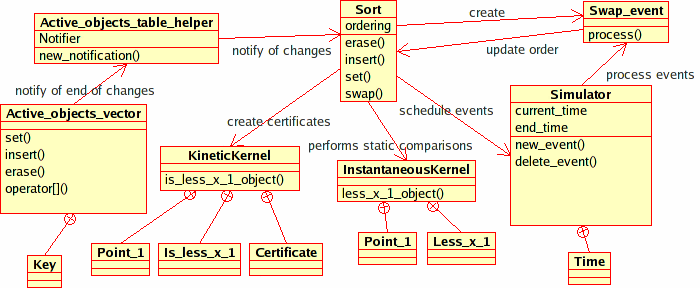
\includegraphics[scale=.8,viewport=0 18 470 250, clip]{Kinetic_data_structures/sort_usage_pct}
\end{center}
\end{ccTexOnly}
\begin{ccHtmlOnly}
<img src="./sort_usage_pct.gif" align=middle alt="Sort Usage"><br>
\end{ccHtmlOnly}
\caption{\label{fig:kds_uml_usage} The figure shows the interaction between
  the \ccc{Kinetic::Sort<Traits, Visitor>} kinetic data structure and
  the various pieces of our package.  Other, more complicated, kinetic
  data structures will also use the \ccc{Kinetic::InstantaneousKernel} in order
  to insert/remove geometric primitives and audit
  themselves. \ccc{Kinetic::Sort<Traits, Visitor>} uses the sorting
  functionality in STL instead.}
\end{figure}

\begin{itemize}

\item the \ccc{Kinetic::Simulator}. Models of this concept process events in
  the correct order and audit kinetic data structures. There should be
  one instance of a model of this concept per simulation.
\item the \ccc{Kinetic::Kernel}. The structure of a
  \ccc{Kinetic::Kernel} is analogous to the static \cgal\ (i.e.,
  non-kinetic) kernels in that it defines a set of primitives and
  functors which generate certificates from the primitives.
\item the \ccc{Kinetic::ActiveObjectsTable}. Models of this concept hold a
  collection of kinetic primitives in a centralized manner. This
  structure centralizes management of the primitives in order to
  properly disseminate notifications when trajectories change, new
  primitives are added or primitives are deleted.
  There is generally one instance of a model of this concept per simulation.
\item the \ccc{Kinetic::InstantaneousKernel}. Models of this concept allow
  existing non-kinetic \cgal\ data structures to be used on a snapshot
  of kinetic data. As a result, pre-existing static structures can be
  used to initialize and audit kinetic data structures.
\item the \ccc{Kinetic::FunctionKernel}. This concept is the computational
  kernel of our framework.  Models of this concept are responsible for
  representing, generating and manipulating the motional and
  certificate functions and their roots. It is this concept that
  provides the kinetic data structures framework with the necessary
  algebraic operations for manipulating event times. The
  \ccc{Kinetic::FunctionKernel} is discussed in detail in Section
  \ref{sec:kds_algebraic_kernel}.
\end{itemize}

For simplicity, we added an additional concept, that of
\ccc{Kinetic::SimulationTraits}, which wraps together a particular set of
choices for the above concepts and is responsible for creating
instances of each of the models. The addition of this concept reduces
the choices the user has to make to picking the dimension of the
ambient space and choosing between exact and inexact computations. The
model of \ccc{Kinetic::SimulationTraits} creates an instance each of the
\ccc{Kinetic::Simulator} and \ccc{Kinetic::ActiveObjectsTable}. Handles for
these instances as well as instances of the \ccc{Kinetic::Kernel}
and \ccc{Kinetic::InstantaneousKernel} can be requested from the simulation
traits class. Both the \ccc{Kinetic::Kernel} and the
\ccc{Kinetic::Simulator} use the \ccc{Kinetic::FunctionKernel}, the former to find
certificate failure times and the later to operate on them. For
technical reasons, each supplied model of \ccc{Kinetic::SimulationTraits} also
picks out a particular type of kinetic primitive which will be used by
the kinetic data structures.


% Both the \object{KineticKernel}
%and the \object{Simulator} query the \object{FunctionKernel} for
%constructing certificate functions, as well as getting their failure
%times.

Surrounding these central set of concepts, there are a large number of
smaller concepts, the models of which act either as glue between
objects or as helper classes.  The key smaller concepts will be described along
with the appropriate central concepts in the corresponding subsections
of Section \ref{sec:kds_architecture}.



